% ============================================================
% LLM-BLM 実験 G：小型株の BLM が効くことの確かめ（G1・G2・G5、寄与、G6、VaR、G3 の検出力。探索）
% コンパイル：tectonic -X compile LLM-BLM_実験G.tex   （XeTeX 系。このフォルダで実行する）
% 数値は experiments/G_proof/results/（summary.json、contrib_summary.json、var.json、power_summary.json、findings.md）
% から写した。図は 作成スクリプト/figs.py。
% ============================================================
\documentclass[xelatex,ja=standard,jafont=haranoaji,a4paper,10pt,openany]{bxjsreport}
\setpagelayout*{left=22mm,right=22mm,top=24mm,bottom=26mm,footskip=11mm}

\usepackage{amsmath,amssymb,mathtools,bm}
\usepackage{booktabs,array,multirow,longtable}
\usepackage{graphicx}
\usepackage{adjustbox}
\usepackage{xcolor}
\usepackage{enumitem}
\usepackage{caption}
\usepackage{float}
\usepackage[most]{tcolorbox}
\usepackage[hidelinks,bookmarksnumbered]{hyperref}

\graphicspath{{図/}}

\definecolor{c1}{HTML}{2A78D6}
\definecolor{c2}{HTML}{EB6834}
\definecolor{c7}{HTML}{6250D6}
\definecolor{soft1}{HTML}{E4EEF9}
\definecolor{soft2}{HTML}{FBEEDF}
\definecolor{soft4}{HTML}{EEE8FA}

\newcommand{\code}[1]{\texttt{#1}}
\newcommand{\figref}[1]{図~\ref{#1}}
\newcommand{\tabref}[1]{表~\ref{#1}}
\newcommand{\chapref}[1]{第~\ref{#1}~章}

\setlist[itemize]{leftmargin=1.6em,itemsep=0.2em,topsep=0.4em}
\setlist[enumerate]{leftmargin=1.8em,itemsep=0.2em,topsep=0.4em}
\captionsetup{font=small,labelfont=bf,skip=6pt}
\renewcommand{\arraystretch}{1.2}

\makeatletter
\def\@makechapterhead#1{\vspace*{0.3\Cvs}{\parindent\z@\raggedright\normalfont
  \ifnum\c@secnumdepth>\m@ne\if@mainmatter{\Large\headfont\@chapapp\thechapter\@chappos}\par\nobreak\vskip0.4\Cvs\fi\fi
  \interlinepenalty\@M\LARGE\headfont #1\par\nobreak\vskip 1.5\Cvs}}
\def\@makeschapterhead#1{\vspace*{0.3\Cvs}{\parindent\z@\raggedright\normalfont
  \interlinepenalty\@M\LARGE\headfont #1\par\nobreak\vskip 1.5\Cvs}}
\makeatother

\newtcolorbox{keybox}[1][要点]{enhanced,breakable,colback=soft1,colframe=c1,boxrule=0.5pt,arc=2pt,
  left=8pt,right=8pt,top=6pt,bottom=6pt,title={#1},fonttitle=\sffamily\bfseries\small,coltitle=white}
\newtcolorbox{notebox}[1][注意]{enhanced,breakable,colback=soft2,colframe=c2,boxrule=0.5pt,arc=2pt,
  left=8pt,right=8pt,top=6pt,bottom=6pt,title={#1},fonttitle=\sffamily\bfseries\small,coltitle=white}
\newtcolorbox{verdict}[1][判定]{enhanced,breakable,colback=soft4,colframe=c7,boxrule=0.5pt,arc=2pt,
  left=8pt,right=8pt,top=6pt,bottom=6pt,title={#1},fonttitle=\sffamily\bfseries\small,coltitle=white}

\title{LLM-BLM 実験 G\\[6pt]
  \large 小型株の BLM が効くことの確かめ\\偽のビュー・ファクター・費用・銘柄の寄与}
\author{実験の報告書（探索。手順は計算の前にコミットで固定）}
\date{2026 年 10 月 27 日}

\begin{document}
\maketitle

\chapter*{概要}
\addcontentsline{toc}{chapter}{概要}

小型株の BLM（S4 の形）は、元と新しい 1,000 社の両方で、比べる相手（範囲の中の会社の浮動株時価総額加重）を上回った（R1 の探索）。この実験 G では、その勝ちが「LLM の読み取り」から来たのか、それとも BLM の仕組み、規模・割安さ・モメンタムへの傾き、一部の銘柄、費用の扱いから来たのかを確かめた。どれも結果を見た後の探索だが、手順と目安は計算の前にコミットで固定した（\code{experiments/G\_proof/plan.md}）。

\begin{keybox}[要点]
\begin{itemize}
\item \textbf{勝ちは LLM の読み取りから来ている（G1）}。点数を銘柄の間で並べ替えた偽物の BLM を 100 回作ると、費用 0.3\% の後で平均は年 $-1.0\%$（元）・$-1.3\%$（新）で、\textbf{本物（年 +2.4\%・+2.2\%）以上は両方の標本で 0 回}（$p$ = 0.01）だった。BLM の仕組みだけでは勝てない。
\item \textbf{ファクターを除いても残る（G2）}。Fama--French の 5 因子とモメンタムで説明できない部分（$\alpha$）は、費用 0.3\% の後で年 +1.9\%（$t$ 2.12、元）・+1.6\%（$t$ 1.65、新）。BLM はモメンタムにはっきり傾いていて、差の約 2 割はそれで説明される。新しい標本の $\alpha$ は目安（片側 $p$ < 0.05）をぎりぎり満たした（$p$ 0.049）。
\item \textbf{費用に弱い（G5）}。これまでの報告（年 +2.9〜3.0\%）は\textbf{費用の前}の値だった。片道 0.3\% の後で年 +2.2〜2.4\%、0.5\% で +1.7〜1.9\%、1\% では有意でない（+0.5〜0.8\%）。BLM は四半期ごとに持ち分の約 85\% を入れ替える。
\item \textbf{寄与は裾に集まるが、一部の銘柄だけではない}。上位 20 銘柄が差の約 9 割を生んだが、下位にも大きな損があり、上下 20 銘柄を両方除いても両方の標本で年 +2.0\% 残った。元の標本では量子コンピュータの IonQ が最大の寄与（差の約 8\%）で、年では 2024 年に偏った。
\item \textbf{単純なポートフォリオでも勝つ（G6）}。同じ条件で点数の上位 20\% を持つだけでも相手を上回ったが、TE は約 6\%（約束の 2 倍）だった。BLM の値打ちは、同じ読み取りを約束のリスク（TE 3\%）の中で使えることにある。
\item 次の段階は、まだ使っていない 400 社での事前登録した検定（G3）。検出力は約 7 割と見積もった。
\end{itemize}
\end{keybox}

\setcounter{tocdepth}{1}
{\small\tableofcontents}

% ============================================================
\chapter{目的}\label{ch:purpose}

総合報告書 3 では、問いを 3 つに分けた。

\begin{enumerate}
\item 決算発表文の読み取りに、小型株の値動きを予測する力があるか（S1・S2、R1 で再現）。
\item それを BLM に入れると、比べる相手に勝てるか（R1 の探索で、両方の標本で年約 +3\%）。
\item 勝った分は LLM の読み取りのおかげか（まだ調べていなかった）。
\end{enumerate}

この実験は、2 と 3 を確かめる。具体的には、\code{やること.md} の G の計画のうち、今のデータでできる G1（偽のビュー）・G2（ファクター）・G5（費用）・G6（単純なポートフォリオとのずれ）と、銘柄ごとの寄与、VaR、G3 の検出力を行った。

% ============================================================
\chapter{方法}\label{ch:method}

\section{共通の設定}

\begin{itemize}
\item 標本：元の 1,000 社（\code{data/smallcap.sqlite}）と、新しい 1,000 社（\code{data/smallcap\_rep.sqlite}）。別々に計算した。
\item ポートフォリオ：S4 の主な形。2015 年末から四半期ごと、ChronoGPT＋リッジの見通し、株価で補正した共分散（B）、TE の上限の校正あり。評価は 2017 年以降の 2,449 日。
\item 株価の誤り：日々のリターンが +300\% 超か $-80\%$ 未満なら欠けとする（R1 の探索の主なしきい値）。
\item \textbf{費用}：計画を書く途中で、S4・R1 の検定に使った日々の超過リターンが\textbf{費用の前}だったことに気付いた（費用は資産の推移にだけ掛かっていた）。そこで、組み直しの日の売買の量を BLM と比べる相手の両方で記録し、片道 $c$ の費用の後の日々の差を「費用の前の差 $- c \times$（BLM の売買の量 $-$ 相手の売買の量）」で計算した。
\item 検定：R1 と同じ、63 日の円形のブロック・ブートストラップ（2,000 回）で、平均 $\le 0$ の割合を片側 $p$ とした。
\item 照合：誤りを除いた費用の前の本物の差は、元 +3.04\%・新 +2.86\% で、R1 の探索の値と一致した。
\end{itemize}

\section{各確かめの中身}

\begin{longtable}{p{2.4cm}p{12.2cm}}
\toprule
\textbf{確かめ} & \textbf{中身} \\
\midrule
\endhead
\bottomrule
\endfoot
G1 偽のビュー & 各組み直しの日に、ビューのある銘柄の点数を、その銘柄の間で並べ替えた BLM を 100 回（seed 0〜99）。どの銘柄にビューがあるか、共分散、$\Omega$、TE の校正、費用は本物と同じ。目安：両方の標本で $p = (1 + \text{本物以上の数}) / 101 < 0.05$ \\
G2 ファクター & 費用 0.3\% の後の日々の差を、Fama--French の 5 因子（市場・規模・割安さ・収益性・投資）とモメンタムに回帰した（日次、2026-08-31 まで 2,428 日、Newey--West のラグ 21）。目安：両方で $\alpha$ の片側 $p < 0.05$ \\
G5 費用 & 片道 0\%・0.3\%・0.5\%・1.0\% で同じ検定 \\
寄与 & 日々の差を、銘柄ごとに（BLM の比率 $-$ 相手の比率）× リターンに分けて足した \\
G6 単純なポートフォリオ & 同じ日程・銘柄・誤りの除き方で、点数の上位 20\% を浮動株時価総額で加重したもの・等金額のもの \\
VaR & 1 日の VaR・CVaR（95\%・99\%、ヒストリカル法と分散共分散法）。記述だけ \\
G3 の検出力 & 使い終わった標本から 400 社を無作為に 10 回ずつ抜き出し、同じ BLM と検定で $p < 0.05$ になる割合 \\
\end{longtable}

% ============================================================
\chapter{結果}\label{ch:results}

\section{G1：偽のビューとの比較}

\begin{verdict}[G1：両方の標本で目安を満たした]
本物以上の偽物は、両方の標本で 100 回のうち 0 回（$p$ = 0.01、100 回で出せる最小）。
\end{verdict}

\begin{table}[H]
\centering\small
\caption{本物と偽物の BLM の、比べる相手との差（年、2017 年以降）。}
\label{tab:g1}
\begin{tabular}{lrr}
\toprule
 & 元の 1,000 社 & 新しい 1,000 社 \\
\midrule
本物（費用 0.3\% の後） & +2.37\% & +2.16\% \\
偽物の平均 & $-0.99\%$ & $-1.26\%$ \\
偽物の 5\%〜95\% 点 & $-2.52$〜+0.45\% & $-2.80$〜+0.33\% \\
本物以上の偽物 & 0 / 100 & 0 / 100 \\
本物 $-$ 偽物の平均 & +3.36\% & +3.42\% \\
費用の前：本物 / 偽物の平均 & +3.04\% / +0.41\% & +2.86\% / +0.16\% \\
\bottomrule
\end{tabular}
\end{table}

\begin{figure}[H]
\centering
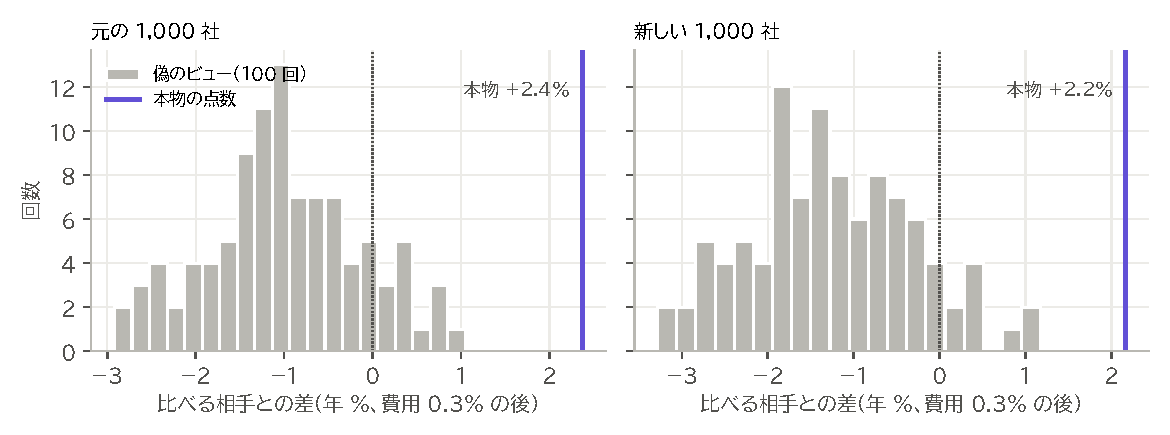
\includegraphics[width=\linewidth]{g1.pdf}
\caption{偽のビューの BLM 100 回の分布と、本物の点数の BLM（費用 0.3\% の後）。}
\label{fig:g1}
\end{figure}

偽物は、費用の前でほぼ 0、費用の後は負けになった。共分散の補正、TE の校正、発表のあった銘柄にだけビューを持つことなど、BLM の仕組みそのものは勝ちを生まない。勝った分は、点数の中身から来ている。

\section{G2：ファクターでの説明}

\begin{table}[H]
\centering\small
\caption{費用 0.3\% の後の日々の差の、5 因子＋モメンタムへの回帰（Newey--West ラグ 21）。}
\label{tab:g2}
\begin{tabular}{lrr}
\toprule
 & 元 & 新 \\
\midrule
同じ日の平均（年） & +2.39\% & +2.09\% \\
\textbf{$\alpha$（年）} & \textbf{+1.94\%（$t$ 2.12、$p$ 0.017）} & \textbf{+1.63\%（$t$ 1.65、$p$ 0.049）} \\
モメンタムの係数 & +0.059（$t$ 12.4） & +0.058（$t$ 7.4） \\
投資（CMA）の係数 & $-0.067$（$t$ $-4.0$） & $-0.061$（$t$ $-3.0$） \\
決定係数 & 0.12 & 0.10 \\
本物 $-$ 偽物の平均の $\alpha$ & +2.81\%（$t$ 2.95） & +2.80\%（$t$ 2.89） \\
\bottomrule
\end{tabular}
\end{table}

BLM は、モメンタム（過去 1 年の勝ち組）を多めに持ち、保守的な投資の会社（CMA）を少なめに持つ方向に傾いていた。差の約 2 割はこの傾きで説明されるが、残りの $\alpha$ は両方の標本で正だった。S1 の探索でも、ドリフトの予測は過去 1 年のモメンタムを統制しても残った（+92.5bp、$t$ 3.81）。

\section{G5：費用}

\begin{table}[H]
\centering\small
\caption{片道の費用ごとの、比べる相手との差（年、95\% 区間、片側 $p$、情報レシオ）。}
\label{tab:g5}
\begin{tabular}{lll}
\toprule
片道の費用 & 元 & 新 \\
\midrule
0\%（S4・R1 の検定） & +3.04\%（+1.22〜+4.93、0.0005、0.97） & +2.86\%（+0.96〜+4.78、0.0005、0.89） \\
\textbf{0.3\%} & \textbf{+2.37\%}（+0.56〜+4.26、0.0075、0.76） & \textbf{+2.16\%}（+0.27〜+4.07、0.013、0.66） \\
0.5\% & +1.93\%（+0.10〜+3.83、0.019、0.61） & +1.70\%（$-0.19$〜+3.61、0.038、0.51） \\
1.0\% & +0.82\%（$-1.03$〜+2.73、0.20、0.25） & +0.53\%（$-1.34$〜+2.44、0.28、0.15） \\
\bottomrule
\end{tabular}
\end{table}

\begin{figure}[H]
\centering
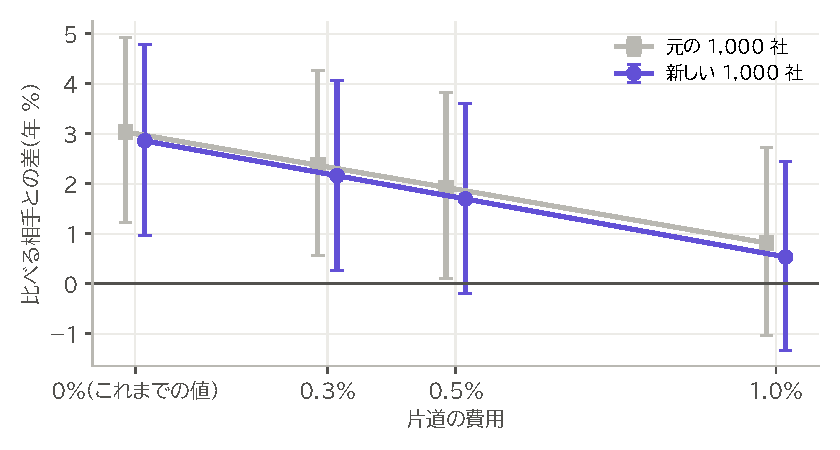
\includegraphics[width=0.75\linewidth]{g5.pdf}
\caption{片道の費用と、比べる相手との差（年）。縦の線は 95\% 区間。}
\label{fig:g5}
\end{figure}

組み直し（四半期）ごとの売買の量（$\sum|\Delta w|$）は、BLM が 0.84〜0.86、比べる相手が 0.28 だった。BLM は毎回、持ち分の大半を入れ替える。小型株で実際の費用が片道 1\% に近いと、勝ちはほぼ消える。

\section{銘柄ごとの寄与}

\begin{table}[H]
\centering\small
\caption{費用の前の差（2017 年以降）の銘柄ごとの内訳。}
\label{tab:contrib}
\begin{tabular}{lrr}
\toprule
 & 元（年 +3.04\%） & 新（年 +3.01\%） \\
\midrule
差がプラスの銘柄 / マイナスの銘柄 & 504 / 489 & 485 / 505 \\
上位 10 銘柄の合計（全体に対する割合） & +1.56\%（51\%） & +1.60\%（53\%） \\
上位 20 銘柄を除いた差 & +0.41\% & +0.24\% \\
上位 20・下位 20 を両方除いた差 & +2.0\% & +2.0\% \\
最大の寄与 & IonQ +0.23\% & Modine +0.21\% \\
量子コンピュータの会社 & IonQ +0.23\%、QUBT $-0.01\%$ & D-Wave ほぼ 0 \\
\bottomrule
\end{tabular}
\end{table}

\begin{figure}[H]
\centering
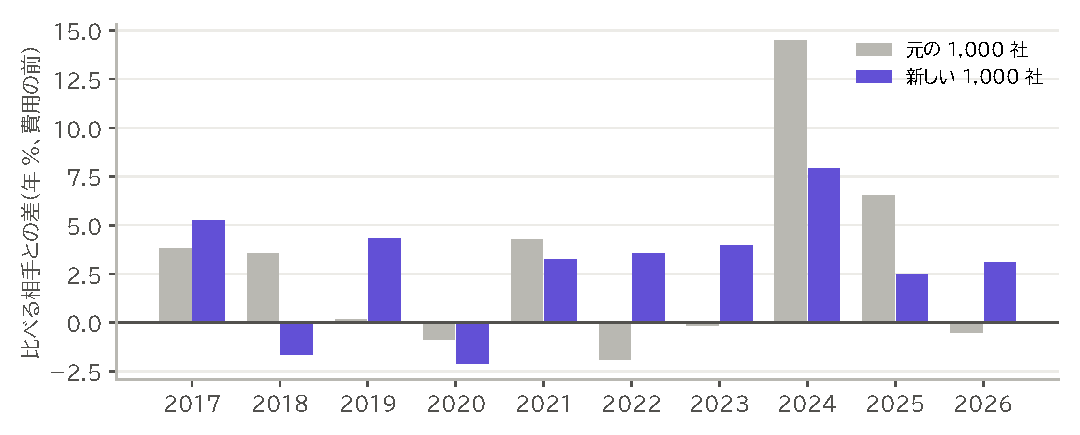
\includegraphics[width=0.95\linewidth]{years.pdf}
\caption{年ごとの、比べる相手との差（費用の前）。2026 年は 8 月まで。}
\label{fig:years}
\end{figure}

差は少数の銘柄の大きな値上がりに偏っている。ただし下位にも大きな損があり、上下を同じ数だけ除くと両方の標本で年 +2.0\% 残った。小型株の能動の運用で寄与が裾に集まるのは普通のことで、「一部の銘柄だけで勝った」とまでは言えない。年ごとに見ると、元の標本は 2024 年（+14.5\%）に大きく偏り、2019〜2023 年はほぼ 0 だった。新しい標本は 10 年のうち 8 年でプラスだった。

\textbf{数値の敏感さ}：新しい標本の寄与の計算では、銘柄の合計が年 +3.01\% で、本物の計算（+2.86\%）とずれた。2016-09-30 の組み直しで比率が変わっていた。同じスクリプトを 2 回走らせると完全に同じだったので、ばらつきではない。足し算の順番などの丸めの違いで、最適化（「解が不正確かもしれない」と警告の出る回）が別の解に移ったものである。BLM の年の差には、この種の数値の敏感さで ±0.15\% ほどの幅がある。

\section{G6：単純なポートフォリオとのずれ}

\begin{table}[H]
\centering\small
\caption{同じ条件（2015 年末から四半期ごと、誤りを除く）での比較。費用 0.3\% の後。どれも寄与の計算（\code{contrib.py}）の値で、新しい標本の BLM は数値の敏感さのため G1 の値（+2.16\%）と少し違う。}
\label{tab:g6}
\begin{tabular}{lll}
\toprule
 & 元：差（片側 $p$、実現の TE、IR） & 新 \\
\midrule
BLM & +2.37\%（0.007、3.1\%、0.76） & +2.29\%（0.009、3.2\%、0.71） \\
上位 20\%・時価総額加重 & +5.20\%（0.003、6.6\%、0.79） & +2.18\%（0.10、5.8\%、0.38） \\
上位 20\%・等金額 & +5.81\%（$<$ 0.001、6.1\%、0.95） & +3.65\%（0.016、6.3\%、0.58） \\
\bottomrule
\end{tabular}
\end{table}

\begin{figure}[H]
\centering
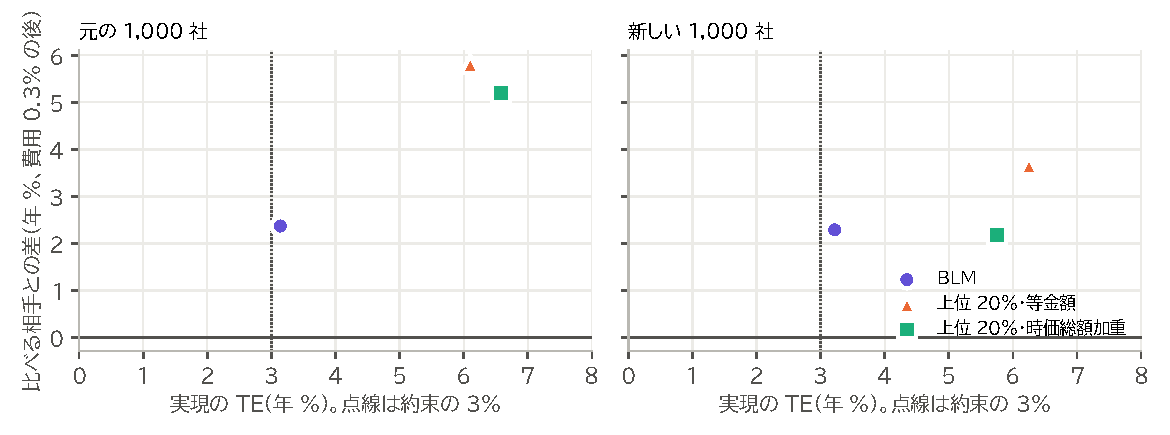
\includegraphics[width=\linewidth]{g6.pdf}
\caption{実現の TE と、比べる相手との差（費用 0.3\% の後）。}
\label{fig:g6}
\end{figure}

S1 の月次の対決（2020 年以降、毎月、上位 20\% を時価総額加重、誤りを除かない）は有意でなかった。条件を BLM にそろえると、単純なポートフォリオでも相手を上回った（元は両方、新は等金額で有意）。読み取りの力は単純な組み方でも出る。ただし TE は約 6\% で、約束の 2 倍だった。BLM は、TE を 3\% に抑えたまま、情報レシオを同じくらいか上（新）に保った。

\section{VaR}

\begin{table}[H]
\centering\small
\caption{1 日の VaR と CVaR（ヒストリカル法、費用 0.3\% の後、2017 年以降）。}
\label{tab:var}
\adjustbox{max width=\linewidth}{\begin{tabular}{lrrrrl}
\toprule
 & 95\% VaR & 95\% CVaR & 99\% VaR & 99\% CVaR & 最悪の日 \\
\midrule
BLM（元） & 2.2\% & 3.4\% & 3.9\% & 5.9\% & $-12.3\%$（2020-03-16） \\
比べる相手（元） & 2.2\% & 3.4\% & 3.7\% & 5.8\% & $-12.3\%$ \\
BLM（新） & 2.2\% & 3.5\% & 4.0\% & 6.2\% & $-14.4\%$（2020-03-16） \\
比べる相手（新） & 2.2\% & 3.5\% & 4.0\% & 6.1\% & $-13.5\%$ \\
相手との差（元 / 新） & 0.30\% / 0.30\% & 0.44\% / 0.45\% & 0.47\% / 0.50\% & 0.70\% / 0.73\% & $-1.8\%$ / $-1.9\%$ \\
\bottomrule
\end{tabular}}
\end{table}

BLM の損の大きさは、比べる相手とほぼ同じだった。BLM が余計なリスクを取っているわけではない。99\% では分散共分散法（BLM で 3.5\%）がヒストリカル法（3.9\%）より小さく、小型株の日々のリターンの裾が正規分布より厚いことを示している。

\section{G3 の検出力}

\begin{table}[H]
\centering\small
\caption{使い終わった標本から 400 社を抜き出した BLM（費用 0.3\% の後）。}
\label{tab:power}
\begin{tabular}{lrrr}
\toprule
抜き出した元 & 差の平均（年） & 平均の IR & $p < 0.05$ の回数 \\
\midrule
元の 1,000 社 & +1.9\% & 0.60 & 9 / 10 \\
新しい 1,000 社 & +1.5\% & 0.47 & 5 / 10 \\
\bottomrule
\end{tabular}
\end{table}

400 社にすると、ビューを持てる銘柄が減り、差は 1,000 社のときより小さくなった。G3（残りの 400 社での事前登録の検定）の検出力は約 7 割である。

% ============================================================
\chapter{考察}\label{ch:discussion}

\section{何が言えるようになったか}

\begin{enumerate}
\item \textbf{問い 3（勝ちは読み取りのおかげか）}：おかげと言える。点数を並べ替えると勝てない（G1）。ファクターを除いても残る（G2）。銘柄の裾を両側から除いても残る（寄与）。
\item \textbf{勝ちの大きさ}：これまでの報告（年約 +3\%）より小さい。費用 0.3\% の後で年 +2.2〜2.4\%、ファクターを除くと +1.6〜1.9\%。
\item \textbf{BLM の役割}：読み取りの力は単純な組み方でも出る。BLM の値打ちは、同じ読み取りを約束の TE の中で使い、損の大きさを比べる相手と同じに保つことにある。
\end{enumerate}

\section{限界}

\begin{itemize}
\item \textbf{探索である}：元と新の標本の結果は、R1 の探索ですでに見ていた。手順は計算の前に固定したが、事前登録した検定ではない。証明は G3 で行う。
\item \textbf{費用}：片道 0.3\% の一定で、売買の量に応じた市場への影響は入れていない。BLM は四半期ごとに持ち分の約 85\% を入れ替えるので、実際の費用が大きいと勝ちは消える。
\item \textbf{生存者バイアス}：今も株価のある会社だけを使っている。比べる相手も同じ会社で作るので差への影響は小さく、残る偏りの主な向き（倒産した会社が抜けること）は結果に不利な側である。上場廃止の株価は取っていない（EODHD の無料版は過去 1 年まで）。
\item \textbf{期間の偏り}：元の標本の差は 2024 年に大きく偏る。
\item \textbf{数値の敏感さ}：最適化の不正確な回で、年の差が ±0.15\% ほど動く。
\item \textbf{訂正}：総合報告書 3 と R1 の報告書の「年約 +3\%」「年 +5.3\%」は費用の前の値である。R1 の事前登録は「費用は S4 と同じ（片道 0.3\%、両方から）」と書いたが、検定に使った系列は費用の前だった。
\end{itemize}

\section{次にすること：G3}

まだ使っていない 400 社（\code{data/smallcap\_g3.sqlite}、データの取得と点数付けは済み、株価の反応は未計算）で、次を事前登録してから 1 回だけ検定する（案は \code{experiments/G3\_confirm/preregistration.md}）。

\begin{itemize}
\item 主な検定：同じ BLM の\textbf{費用 0.3\% の後}の差の平均 > 0（片側 $p$ < 0.05）。
\item 誤りを除く規則（+300\%・$-80\%$）と費用の扱いは、この実験と同じに固定する。
\item 検出力は約 7 割なので、「支持されない」は「効かない」の証拠にならないと先に書いておく。
\end{itemize}

\begin{notebox}[追記（2026-10-27）：G3 の結果]
G3 を事前登録（コミット \code{4bec5c4}）してから 1 回だけ計算した。費用の後の差は年 +0.74\%（95\% 区間 $-1.24$〜+2.86\%、片側 $p$ 0.252）で、\textbf{支持されなかった}。偽のビューは 100 回中 12 回が本物以上（$p$ 0.13）、因子の $\alpha$ は +0.51\%（$t$ 0.46）。G3 ではドリフトの予測（S1）も支持されず（+23.8bp/SD、$t$ 0.66）、変動率の予測（S2）は支持された（$t$ 4.38）。この実験で見た元・新の標本での勝ちは、まだ使っていない会社では確かめられなかった。詳しくは総合報告書 3 の第 VI 部と \code{experiments/G3\_confirm/results/findings.md}。
\end{notebox}

% ============================================================
\chapter*{再現の手順}
\addcontentsline{toc}{chapter}{再現の手順}

リポジトリの直下で（\code{.venv} の Python）：

\begin{enumerate}
\item \code{python experiments/G\_proof/run.py orig real}、\code{... rep real}（本物。約 20 分）。
\item \code{python experiments/G\_proof/run.py orig shuffle 0 20} など、seed 0〜99 を分けて並列に（偽物。1 回 2〜9 分）。
\item \code{python experiments/G\_proof/analyze.py}（G1・G2・G5 → \code{results/summary.json}）。
\item \code{python experiments/G\_proof/contrib.py orig}、\code{... rep}（寄与と G6、各 2 分）。
\item \code{python experiments/G\_proof/var.py}、\code{python experiments/G\_proof/power.py orig power 0 5} など。
\item このフォルダの \code{作成スクリプト/figs.py} と \code{tectonic -X compile LLM-BLM\_実験G.tex}。
\end{enumerate}

計画と結果の記録は \code{experiments/G\_proof/plan.md} と \code{results/findings.md}。

\end{document}
